\documentclass[14pt]{article}
\usepackage{url}
\usepackage{hyperref}
\usepackage{amsmath}
\usepackage{mathtools}
\usepackage{extsizes}
\usepackage{titling}
\usepackage{siunitx}
\usepackage{graphicx}
\usepackage[font=small,labelfont=bf]{caption}
\usepackage[shortlabels]{enumitem}
\usepackage[margin=0.8in]{geometry}


\newcommand{\bd}{\textbf}

\setlength{\droptitle}{-5em} 

\title{Written Homework 1}
\author{Mitchell Meier}
\date{\today}

\begin{document}

\maketitle

\begin{enumerate}

\item

\begin{enumerate}[(a)]

\item
\begin{itemize}
\item \bd{Name of individual} is qualitative nominal 
\item \bd{Systolic blood pressure} is quantitative discrete (at least in this data set) 
\item \bd{Age in years} is qualitative discrete 
\item \bd{Weight in pounds} is qualitative discrete (at least in this data set where it is rounded, is usually a qualitative ordinal value) 
\item \bd{Smoking/Nonsmoking} is qualitative nominal 
\item \bd{Level of physical activity} is qualitative ordinal in this study (goes from bottom to top poor, normal, good, excellent) 
\end{itemize}

\item
For the analysis of the recorded data, I am going to analyze the summaries of the numerical data, analyze the coorelation between age and systolic blood pressure, and analyze the coorelation between physical activity and systolic blood pressure 

\subsection*{Nummerical Analysis}

When looking at the numerical variables in this survey, I believe the first thing to do is too make sure the individuals picked for the sample are a good representation of the survey's population. The prompt did not specifically state the population, but based on the mean age of the sample being 62 years old, I belive the survey aimed to study people between middle aged and seniors. There are a couple outliers in the sample, but looking at the Interquartile Range for age, it shows that three fourths of the individuals were between 54 and 74, with only a few outliers below that \pagebreak

\begin{figure}[h]
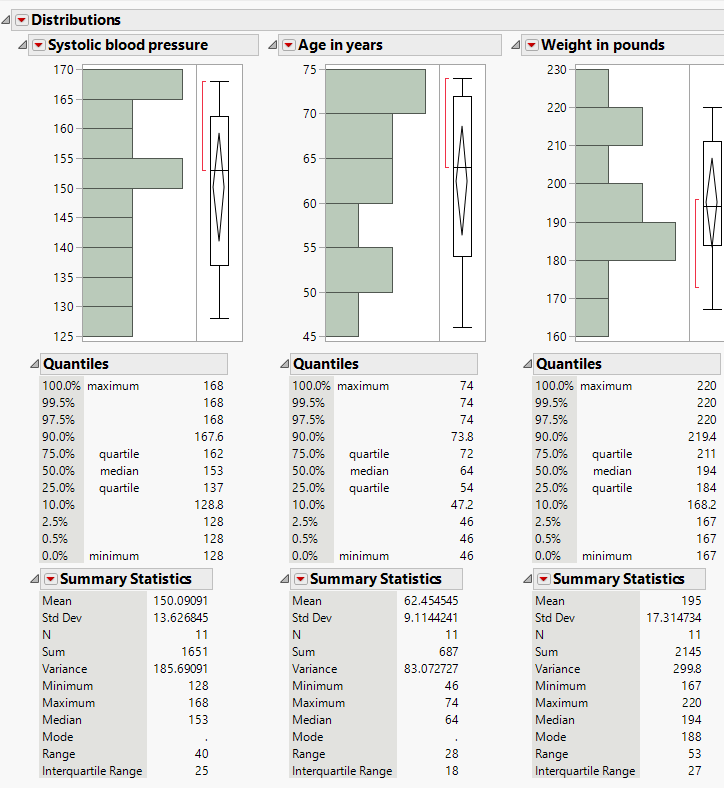
\includegraphics[scale=0.75]{hw1Pics/NumericalAnalysis.PNG}
\centering
\caption{Summaries of the data in each numerical column of the survey}
\end{figure}

So now that we have an idea of what age group we are looking at, does the weight of this sample accuratley represent that population? To determine that, it would be best to split up data between men and women. This is an assumption, but based on the names recorded there are most likely 6 males and 5 females, with the average weight for males being 195.5 pounds and the average weight for females being 194.4. For the male number, that value is within one pound of the american average for men at age 65 (194.7 pounds), so that is an exceptionally accurate sample for the population. However, the average weight for females in america aged 65 is 166.5 pounds, so our sample size here may give us an accurate representation of systolic blood pressure for women in our age range. And for the age values in general, it is noteworthy to point out that the standard devation value is 17.3, much higher than the other two numeric variables, meaning that the variance between values in our weight column is quite high, and certain data points may not be an accurate representation of the mean  \\

\begin{figure}[h]
\captionsetup{justification=centering}
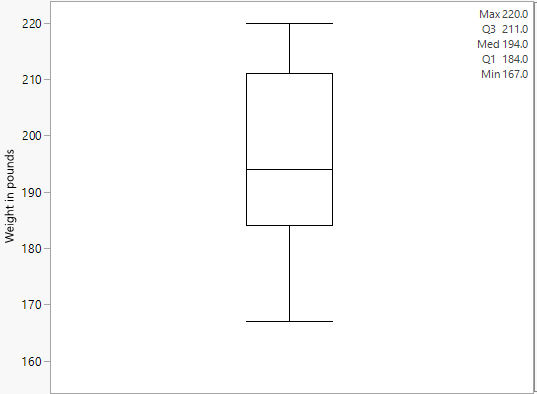
\includegraphics[scale=0.75]{hw1Pics/weightboxplot.PNG}
\centering
\caption{Boxplot of our sample's weight variable, \\ showing the comparitivley high variance compared to our other variables}
\end{figure}

For the systolic blood pressure variable, since that is the response variable we are testing, I will save analysis on that for my section, where I show how certain other columns in the survey effect our response variable's value \\

\subsection*{Coorelation Analysis}

The two coorelations I want to look into, because I think they are the strongest coorelations in the survey, are the coorelations between systolic blood pressure and age, and the coorelation between systolic blood pressure and physical activity \pagebreak

Looking at a line graph comparing systolic blood pressure to age, there's an obvious coorelation between high blood pressure and old age. The reason I pointed out this coorelation is because I think it's an easy argument to say that old age causes high blood pressure. It's certain that blood pressure is the response variable in this scenario, because we know that age is not influenced by anything but time (for example, your age is guaranteed to not increase suddenly if your blood pressure increases suddenly). Out of all the variables in the survey, age has the strongest coorelation with systolic blood pressure \\

\begin{figure}[h]
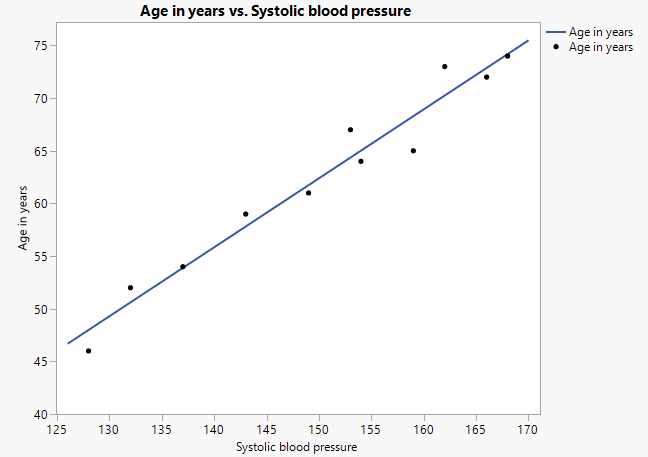
\includegraphics[scale=0.75]{hw1Pics/agevsbplinegraph.PNG}
\centering
\caption{Line graph of age in years vs systolic blood pressure, with a best fit line}
\end{figure}

\pagebreak

Moving onto the next graph, we have replaced the age variable with the level of physical activity each individual has. The conclusion here, while not as strong as the last graph, are pretty conclusive that better physical activity results in lower blood pressure. The reason our conclussion here is not as strong is because the coorelation between physical activity and blood pressure could be a spurious coorelation. It is true that when an individual's quality of activiy increases, their blood pressure decreases, but the reason that an indivudual's quality of activiy increases could be many different variables. For instance, a person who is younger might have a higher quality of physical activity since it is usually easier for them to excersice. The fact that there could be this third factor that happens to be coorelated to both our current variables tells us it is not certain that quality of phyiscal activity and blood pressure are directly coorelated \\


\begin{figure}[h]
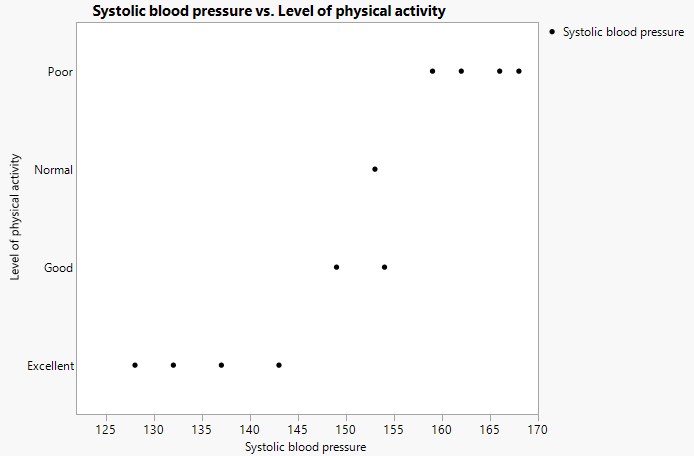
\includegraphics[scale=0.75]{hw1Pics/bpvsphysactivity.PNG}
\centering
\caption{Graph that plots the comparison between systolic blood pressure and physical activity}
\end{figure}

\pagebreak

\end{enumerate}

\item
\bd{I - Individual} 

The individual in this survey is the student. The surveryors are analyzing a trait that the S\&T student has \\

\bd{V - Variable} 

The variable in this survey is the opinion on online classes. The student's preference on fully online classes is the piece of information the surveyors are recording \\

\bd{P - Population} 

I believe the population is the S\&T community, since the prompt mentions that the survey includes the entire S\&T community. Even though this survey is only focusing on students, it most likely is just a part of a study focused on the S\&T community as a whole. If it is not, then the population would just be students \\

\bd{P - Parameter} 

The parameter for this survey is the proportion of students who prefer fully online classes. Meaning they want to know that a student either prefers or does not prefer fully online classes, then keep a running tally of each to compare them \\

\bd{S - Sample} 

The sample, or subset of the population, that the surveyors chose was 100 students from S\&T \\

\bd{S - Statistic} 

The statistic for this survey would be the proportion of S\&T students (out of the 100 in the sample) who prefer fully online classes \\



\item

\begin{enumerate}[(a)]

\item
The \bd{response variable} is the observed battery life that results from the battery being subjected to a certain material type and temperature 

\item 
The \bd{factors} are material type and temperature. The \bd{factor levels} for material type are listed as material 1, 2, and 3, and the levels for the temerature are 15\si{\degree}F, 70\si{\degree}F, and 125\si{\degree}F 

\item
The number of \bd{treatment combinations}, or different combination of factors is $3^2 = 9$, since there are 3 levels per factor, and two total factors. The \bd{treatment conditions} are: \\

MType 1 and 15\si{\degree}F, MType 1 and 70\si{\degree}F, MType 1 and 125\si{\degree}F \\
MType 2 and 15\si{\degree}F, MType 2 and 70\si{\degree}F, MType 2 and 125\si{\degree}F \\
MType 3 and 15\si{\degree}F, MType 3 and 70\si{\degree}F, MType 3 and 125\si{\degree}F \\

\item
The number of \bd{replications} total is the number of treatment combinations (9) times the number of replications each treatment combination recieves (4)
\[
9 \times 4 = 36
\]
which gives us 36 total replications 

\end{enumerate}

\end{enumerate}

\end{document}